\subsection{Architecture physique}

Le diagramme ci-dessous représente l'architecture physique du programme {\nomLogiciel} et de l'application {\nomApplication} dans leur intégralité. En plus des
classes vues précédemment, ce diagramme présente la gestion de la communication ainsi que les objets frontières nécessaires au bon fonctionnement du système.
Dans ce diagramme, dans un souci de visibilité, nous avons décidé de ne pas détailler les opérations ainsi que les attributs des classes.

\begin{minipage}
    {\linewidth}
    \centering
    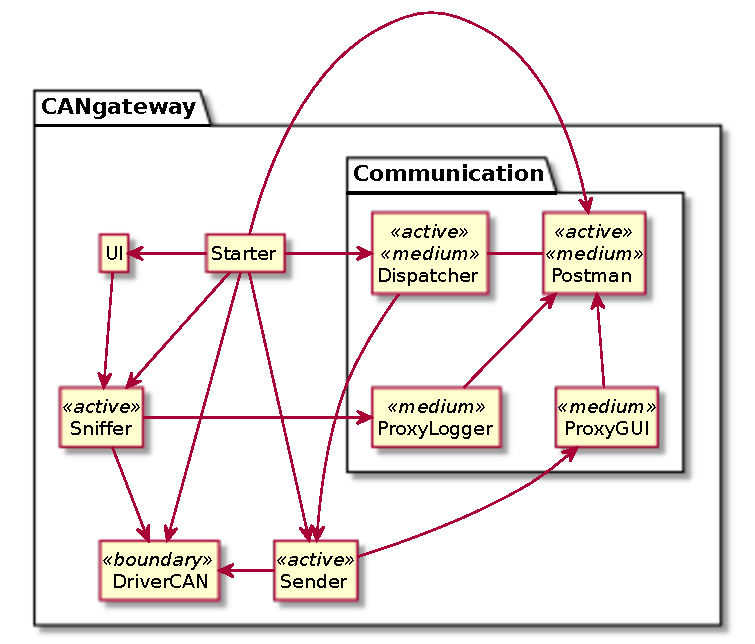
\includegraphics[width=0.8\textwidth]{../schemas/Conception_detaillee/architecture_CANgateway.pdf}
    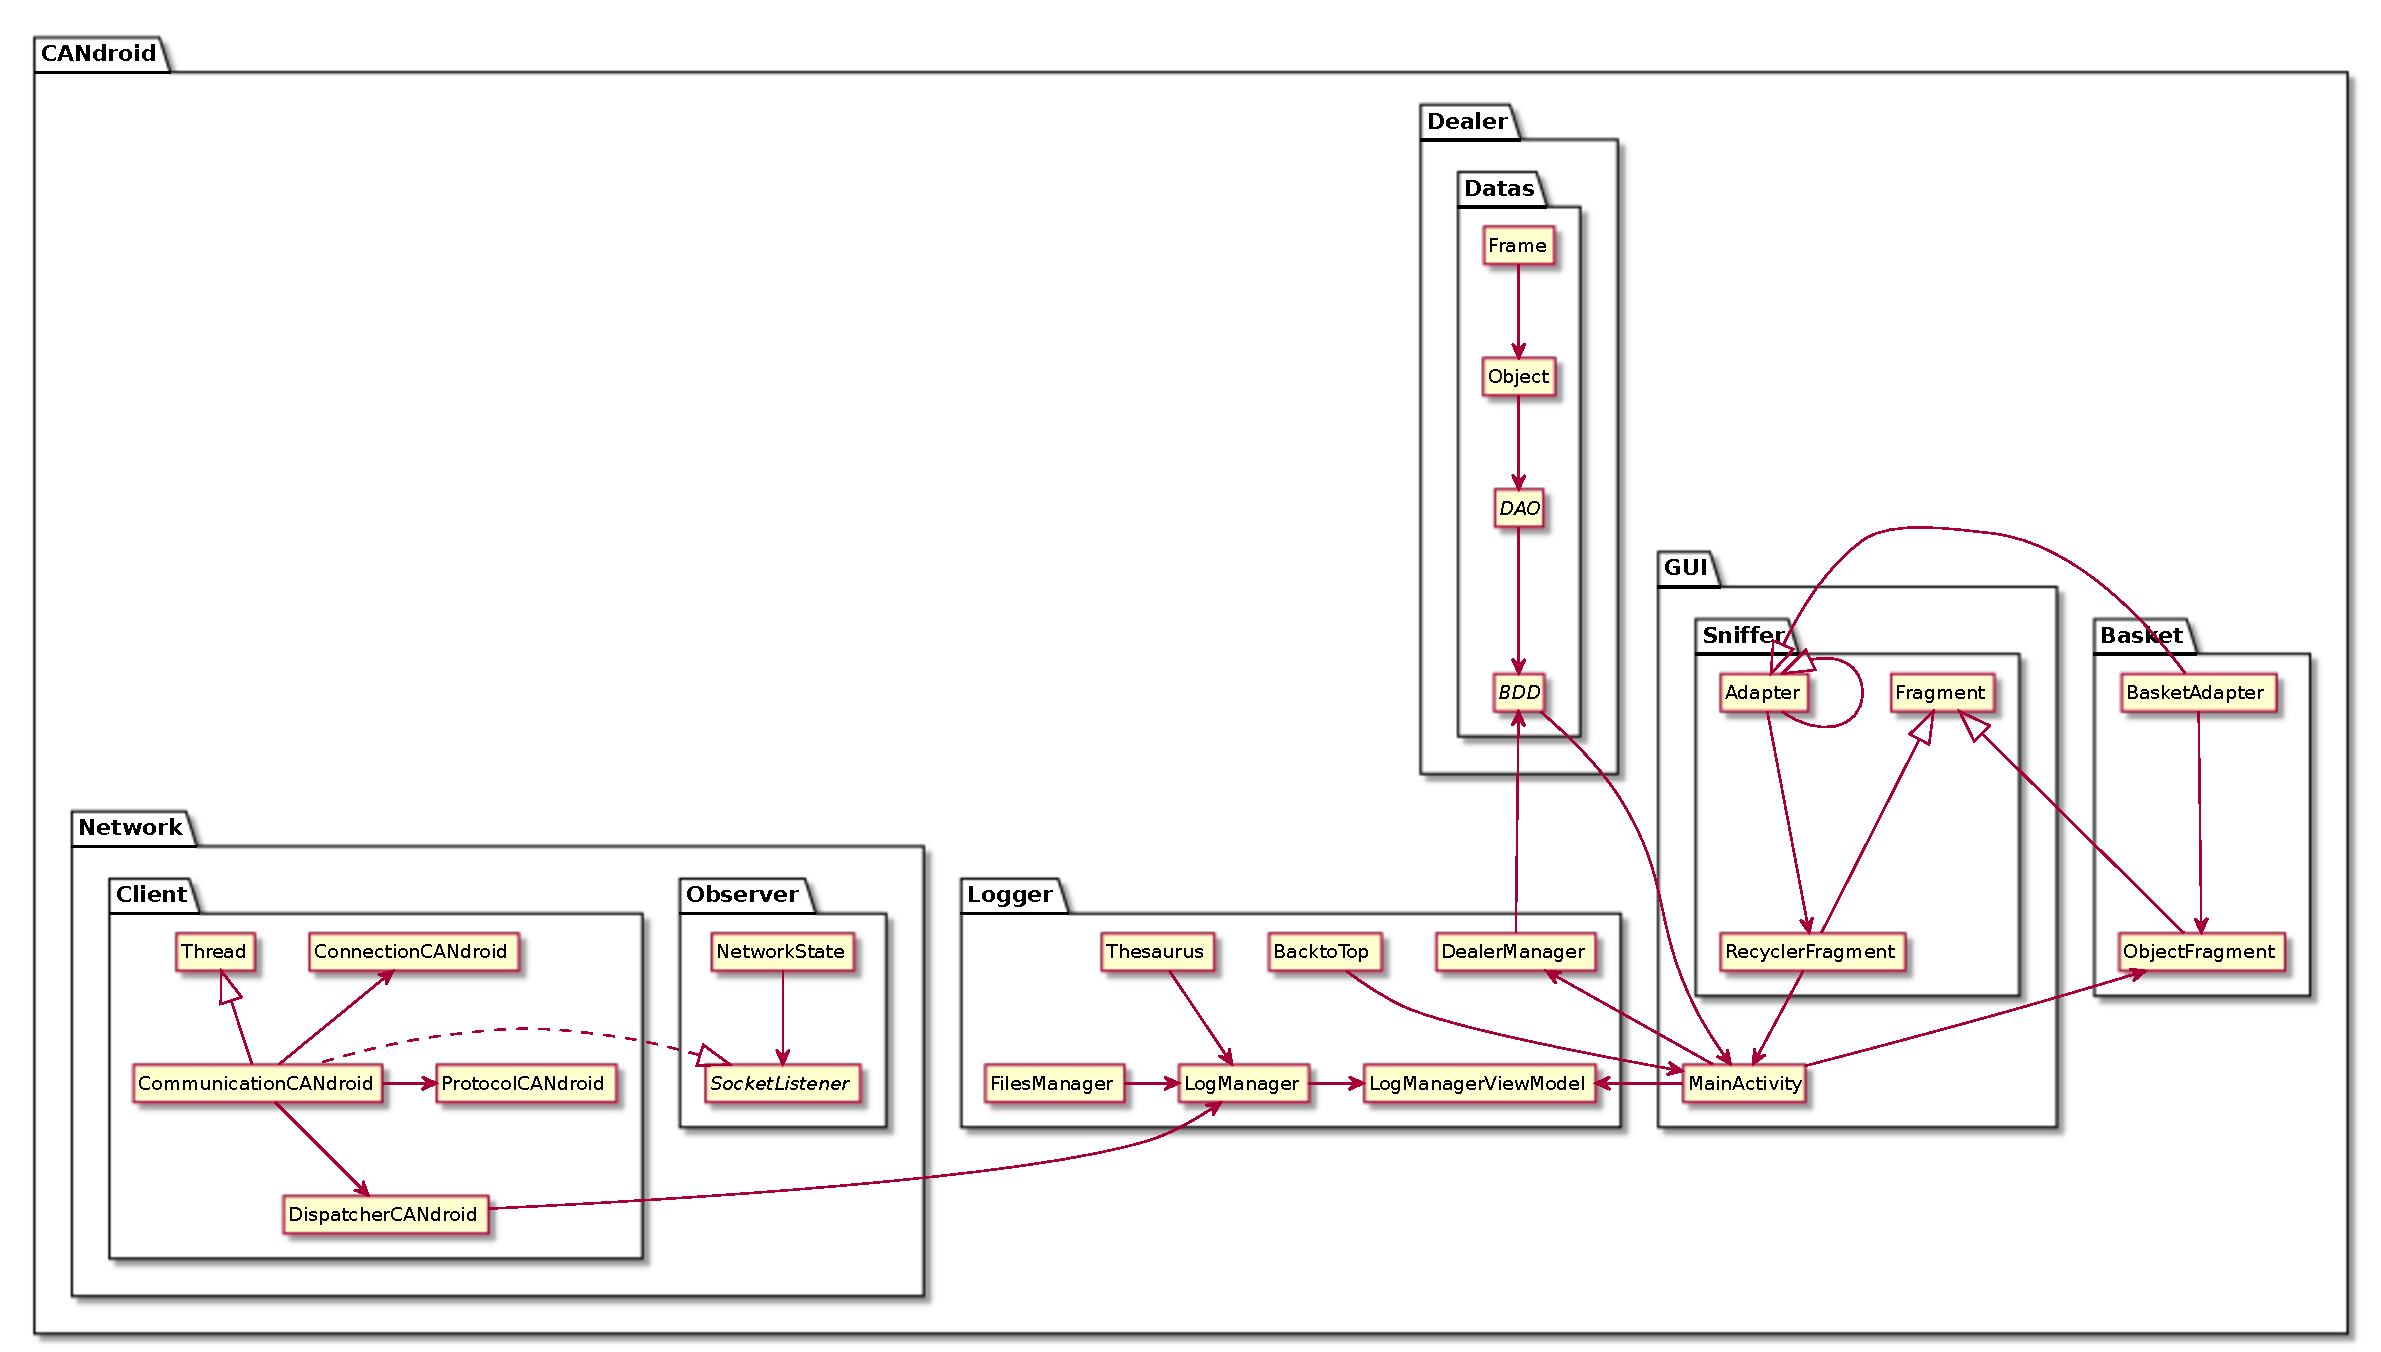
\includegraphics[width=\textwidth]{../schemas/Conception_detaillee/architecture_CANdroid.pdf}
    \captionof{figure}{Architecture physique}
\end{minipage}